\begin{figure}
\begin{center}
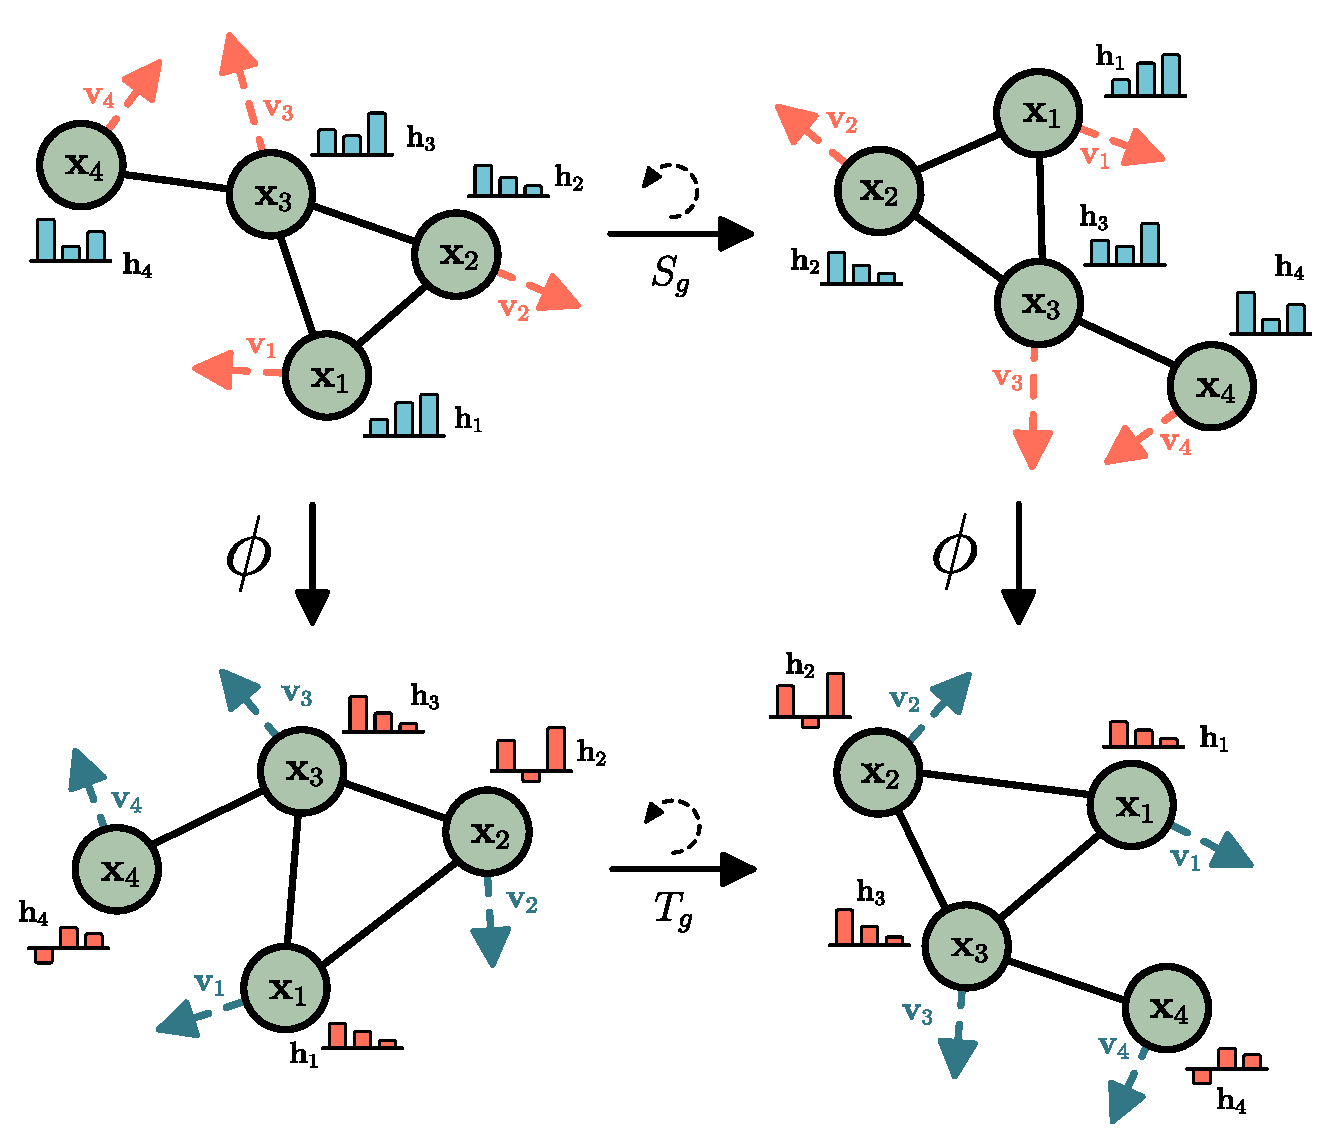
\includegraphics[width=0.99\columnwidth]{Figures/overview_equivariance.pdf}
\caption{Example of rotation equivariance on a graph with a graph neural network $\phi$}
\label{fig:overview_equivariance}
\end{center}
\end{figure}
\vspace{-5pt}

\section{Introduction}
% Equivariance is cool
Although deep learning has largely replaced hand-crafted features, many advances are critically dependent on inductive biases in deep neural networks. An effective method to restrict neural networks to relevant functions is to exploit the \textit{symmetry} of problems by enforcing equivariance with respect to transformations from a certain symmetry group. Notable examples are translation equivariance in Convolutional Neural Networks and permutation equivariance in Graph Neural Networks \cite{bruna2013spectral, defferrard2016convolutional, kipf2016semi}. 

% Still needs editing.
Many problems exhibit 3D translation and rotation symmetries. Some examples are point clouds \cite{uy2019revisiting}, 3D molecular structures \cite{ramakrishnan2014quantum} or N-body particle simulations \cite{kipf2018neural}. The group corresponding to these symmetries is named the Euclidean group: SE(3) or when reflections are included E(3). It is often desired that predictions on these tasks are either equivariant or invariant with respect to E(3) transformations.

% SE(3) equivariance is cool, studies focus on higher types representations.
Recently, various forms and methods to achieve E(3) or SE(3) equivariance have been proposed \cite{thomas2018tensor, fuchs2020se, finzi2020generalizing, kohler2020equivariant_icml}. Many of these works achieve innovations in studying types of higher-order representations for intermediate network layers. However, the transformations for these higher-order representations require coefficients or approximations that can be expensive to compute. Additionally, in practice for many types of data the inputs and outputs are restricted to scalar values (for instance temperature or energy, referred to as type-$0$ in literature) and 3d vectors (for instance velocity or momentum, referred to as type-$1$ in literature). 
% In \cite{thomas2018tensor,fuchs2020se} the higher type representations are transformed according to the spherical harmonics which need to be recomputed for each datapoint and can be expensive.


% A big part of the current deep learning advances come from inductive baises. A successful way to include inductive biases in deep learning models is by exploiting the symmetries of the data using equivariant functions. Equivariance has proven his success in a variety of applications, for example, Convolutional Neural Networks (CNNs) are translation equivariant, which means that a translation of the input image corresponds to an equivalent translation of the output feature map. This discards the need to do data augmentation reducing the computating resouces in terms of training time and model capacity. Equivariance can also be found in other successful cases like permutation equivariance in Graph Neural Networks 

% Other directions


In this work we present a new architecture that is translation, rotation and reflection equivariant ($\En$), and permutation equivariant with respect to an input set of points. Our model is simpler than previous methods in that it does not require the spherical harmonics as in \cite{thomas2018tensor, fuchs2020se} while it can still achieve competitive or better results. In addition, equivariance in our model is not limited to the 3-dimensional space and can be scaled to larger dimensional spaces without a significant increase in computation. 

We evaluate our method in modelling dynamical systems, representation learning in graph autoencoders and predicting molecular properties in the QM9 dataset. Our method reports the best or very competitive performance in all three experiments.